% CVPR 2025 Paper Template; see https://github.com/cvpr-org/author-kit

\documentclass[10pt,twocolumn,letterpaper]{article}

%%%%%%%%% PAPER TYPE  - PLEASE UPDATE FOR FINAL VERSION
\usepackage{cvpr}              % To produce the CAMERA-READY version
% \usepackage[review]{cvpr}      % To produce the REVIEW version
% \usepackage[pagenumbers]{cvpr} % To force page numbers, e.g. for an arXiv version

% Import additional packages in the preamble file, before hyperref
\input{preamble}

% It is strongly recommended to use hyperref, especially for the review version.
% hyperref with option pagebackref eases the reviewers' job.
% Please disable hyperref *only* if you encounter grave issues, 
% e.g. with the file validation for the camera-ready version.
%
% If you comment hyperref and then uncomment it, you should delete *.aux before re-running LaTeX.
% (Or just hit 'q' on the first LaTeX run, let it finish, and you should be clear).
\definecolor{cvprblue}{rgb}{0.21,0.49,0.74}
\usepackage[pagebackref,breaklinks,colorlinks,allcolors=cvprblue]{hyperref}
\usepackage{tikz}
\usepackage{pgfplots}
\pgfplotsset{compat=1.18}
\usepackage{anyfontsize}
\usepackage{tcolorbox}
\usepackage{xcolor}
\usepackage{caption}

%%%%%%%%% PAPER ID  - PLEASE UPDATE
\def\paperID{*****} % *** Enter the Paper ID here
\def\confName{CVPR}
\def\confYear{2025}

%%%%%%%%% TITLE - PLEASE UPDATE
\title{
Diffusion Policy: Visuomotor Policy Learning via Action Diffusion\\
\textit{Article Study}
}

%%%%%%%%% AUTHORS - PLEASE UPDATE
\author{
Lounès Meddahi\\
ENS Rennes\\
MVA, ENS Paris-Saclay\\
{\tt\small lounes.meddahi@ens-paris-saclay.fr}
% For a paper whose authors are all at the same institution,
% omit the following lines up until the closing ``}''.
% Additional authors and addresses can be added with ``\and'',
% just like the second author.
% To save space, use either the email address or home page, not both
\and
Tom Ravaud\\
ENPC\\
MVA, ENS Paris-Saclay\\
{\tt\small tom.ravaud@enpc.fr}
}

\begin{document}

\maketitle
\begin{abstract}

Diffusion policy is a visuomotor policy that leverages the latest advances in diffusion models to perform
complex manipulation tasks from human demonstrations.
More specifically, it involves denoising a sequence of actions to be performed, conditioned on the visual
observation of the scene. The use of diffusion provides a real advantage to the approach, enabling it
to surpass previous methods. In this study, we aim to understand what motivated the development of this
approach, reproduce the reported results, and explore its limitations.

\end{abstract}
\section{Introduction}
\label{sec:intro}

Robotics has traditionally been state-based, meaning we attempt to estimate the state of a dynamic system
from our sensor measurements and construct the action to perform based on this state.
Today, mainly due to technical advances in deep learning, it has become common to bypass this intermediate
representation and directly construct the action from the observation, using sensor-based approaches.
A visuomotor policy refers to a policy that generates actions based on
visual observations of the scene.
An early example of such a policy can be obtained by image-based visual servoing,
where the goal is to move the robot so that its observation matches a target observation
(for example, by overlaying local correspondences between the two images) \cite{chaumette_visual_2006}.
However, we are quickly limited to simple positioning tasks.
Imitation learning is a popular framework for designing
such a policy in the context of complex robotic manipulation, as it enables learning from human demonstrations
in a supervised way \cite{florence_implicit_2021,zhao_learning_2023}.

\vspace{0.5em}
Multiple challenges arise in this setting:
\begin{itemize}
    \item \textbf{Action multimodality}. How to handle situations where different actions are equivalent?
    \item \textbf{Temporal consistency} of the generated actions. How to ensure a smooth trajectory?
    \item \textbf{High-dimensional action space}. How to scale up?
\end{itemize}

\vspace{0.5em}
Several approaches have addressed the problem of action multimodality.
The idea is always the same: to sample an action from the (potentially multimodal) distribution of
possible actions at the current moment to perform the task.
This distribution can be explicitly predicted by discretizing the action space \cite{shafiullah_behavior_2022} or
using a Gaussian mixture \cite{mandlekar_what_2021}.
Today, generative models allow for better capturing of multimodality by implicitly learning the
underlying distribution. In the literature, approaches include energy-based models \cite{florence_implicit_2021},
conditional variational autoencoders (VAEs) \cite{zhao_learning_2023}, or diffusion models \cite{chi2023diffusion}.
Regarding temporal consistency, receding-horizon-like strategies have proven to be effective but require
the model to be able to predict a sequence of actions, which can be of high dimension.

\vspace{0.5em}
DiffusionPolicy (DP) \cite{chi2023diffusion} is a candidate solution that addresses theses challenges:
It leverages conditioned diffusion models to sample from an unknown complex and
multimodal distribution of action sequences, and a receding-horizon control strategy.

\section{Method}
\label{sec:method}


There are different diffusion frameworks, including DDPM \cite{ho_denoising_2020} and
DDIM \cite{song_denoising_2022}, which involve a denoising network $\varepsilon_\theta$ whose
architecture is generally independent of the diffusion parameters. We will focus more on the network
architecture than on the diffusion process itself, as no contribution is made to the latter. Note that
the authors of the paper used the DDIM framework so as to be able to use a different number of denoising
iterations in training and inference, which allows for a faster sampling process at test time.

At timestep t, let $A_t$ be the action sequence and $O_t$ the observation.
% (which may contain several previous images of the scene and the end-effector pose).
The observation may contain features from several previous images of the scene, extracted by a trainable
ResNet encoder, and the end-effector pose. This observation vector is seen as a conditioning input
to guide the action sequence generation. Once the action sequence is generated, the agent executes only a
subset of it, in a receding horizon fashion.
Two architectures are proposed for the denoising network (Figure \ref{fig:diffusion_policy}).
\begin{figure*}
    \centering
    \includegraphics[width=\linewidth]{figures/policy_input_output.pdf}
    \caption{a) Denoising network overview, b) CNN-based and c) Transformer-based architectures.}
    \label{fig:diffusion_policy}
\end{figure*}
The first model is a 1D U-Net composed of strided and transposed convolutions, with conditioning
incorporated through FiLM layers. The second model includes attention layers and uses cross-attention
for conditioning.
The integration of the network within the diffusion process is shown in Figure \ref{fig:diffusion}.

\begin{figure}
    \centering
    \includegraphics[width=\linewidth]{figures/diffusion.pdf}
    \caption{Diffusion involves training the network to denoise noisy action sequences,
    in order to be able to sample sequences from pure noise during inference.}
    \label{fig:diffusion}
\end{figure}
\begin{table}[!htb]
    \centering
    \begin{tabular}{c|c}
        \textbf{Method} & max / avg \\
        \hline
        LSTM-GMM & 0.69/0.54 \\
        IBC & 0.75/0.64 \\
        \textbf{DP-CNN} & \textbf{0.91}/\textbf{0.84} \\
        \textbf{DP-Transformer} & 0.78/0.66
    \end{tabular}
    \caption{Success rate in the PushT environment. The goal of the agent is to push a T-shaped
    block to a fixed target. The CNN version of DP outperforms its competitors.}
    \label{tab:success_rate}
\end{table}
The approach is evaluated on the PushT environment (Table \ref{tab:success_rate}).
DP has proven to be capable of modeling multimodal distributions (Figure \ref{fig:multimodality}).
\begin{figure}
    \centering
    \fbox{\includegraphics[width=\linewidth]{figures/multimodal_sim.pdf}}
    \caption{Ability of different approaches to handle multimodality. The agent (blue) must push the
    object (grey) to the target (green). In this specific case, the agent should be able to bypass the
    T-shaped obstacle by the left or right.}
    \label{fig:multimodality}
\end{figure}

\section{Experiments} \label{sec:experiments}
In this section, we present our test-time experimental setup used to evaluate the DP framework under varying conditions
and introduce some points of discussion we found relevant and decided to explore further.

In Section~\ref{sec:pretrained_model}, we begin by describing the pre-trained LeRobot model we use for the Push-T environment.
We then detail how we managed to train our own models from scratch in Section~\ref{sec:training_model}.
In Section~\ref{sec:tradeoff_denoising_steps}, we briefly discuss the trade-off between the number of denoising
steps and the model's performance.
Next, in Section~\ref{sec:action_multimodality}, we investigate the agent's behavior in multimodal scenarios, where multiple valid action trajectories are possible (e.g. bypass the T by the left or right).
Finally, in Section~\ref{sec:visual_perturbations}, we detail the evaluation protocols and experimental setup used to introduce and measure the impact of visual perturbations on the policy's performance.

\subsection{LeRobot's Pre-Trained Action Diffusion Model}\label{sec:pretrained_model}

While the authors of the original DP article have made their code available, a recent and more
accessible implementation has been provided by Hugging Face through their LeRobot
framework~\cite{cadene2024lerobot}.

Our first experiments were based on a pre-trained diffusion policy model provided by the LeRobot team
and applied to the Push-T environment
\footnote{Available at \url{https://github.com/huggingface/gym-pusht}}.
The goal of this task is to push a T-shaped block to a fixed target location in a 2D space. There are two
ways of assessing the agent's performance: the success rate and the average maximum overlap between the
object and the target. To be considered successful, the object must overlap the target by at least 95\%.

While the original DP authors proposed two implementations, a Transformer-based and a CNN-based architecture,
only the latter is available in the LeRobot library.
Visual observations are processed using a ResNet-18 encoder trained from scratch (i.e., without ImageNet
pretraining), transforming raw RGB inputs into compact feature vectors.
These observation features condition the diffusion process that sequentially predicts actions, which are
end-effector positions.
This diffusion-based policy has been trained from 206 human demonstrations
\footnote{Collected via \url{https://github.com/real-stanford/diffusion_policy}}, for 7 hours on
an Nvidia RTX 3090.
More precisely, it consists of 200k steps of training with a batch size of 32, using various data
augmentation techniques (image brightness, contrast, saturation, hue and sharpness).

Figure~\ref{fig:coverage_illustration} illustrates three possible outcomes with different object-to-target
coverage levels.
\begin{figure}[!htb]
    \centering
    \begin{subfigure}[b]{0.4\linewidth}
        \centering
        \includegraphics[width=\linewidth]{figures/illustration_0.pdf}
        \caption{No coverage ($\approx 0.0\%$)}
    \end{subfigure}

    \begin{subfigure}[b]{0.4\linewidth}
        \centering
        \includegraphics[width=\linewidth]{figures/illustration_50.pdf}
        \caption{Low coverage ($\approx 16\%$)}
    \end{subfigure}
    \begin{subfigure}[b]{0.4\linewidth}
        \centering
        \includegraphics[width=\linewidth]{figures/illustration_150.pdf}
        \caption{High coverage ($\approx 89\%$)}
    \end{subfigure}
    \caption{Illustrations of different object-to-target coverage levels obtained by the LeRobot pre-trained diffusion policy on the Push-T task.}
    \label{fig:coverage_illustration}
\end{figure}
The evaluation results\footnote{Available at \url{https://huggingface.co/lerobot/diffusion_pusht}} of
the LeRobot's implementation compared to a CNN-based architecture similar to the original DP article are
summarized in Table~\ref{tab:evaluation_results}.
\begin{table}[!htb]
    \centering
    \begin{tabular}{lcc}
    \hline
    Metric & HF & DP \\
    \hline
    Average max. overlap (\%) & 95.9 & 95.7 \\
    Success rate (\%) & 63.8 & 64.2 \\
    % Beta distribution lower/mean/upper (\%) & 61.6 / 63.7 / 65.9 & 62.0 / 64.1 / 66.3 \\
    \hline
    \end{tabular}
    \caption{Evaluation results of the pre-trained diffusion policy model (`DP') compared to the LeRobot implementation (`HF'). Metrics are computed over 500 evaluation episodes.}
    \label{tab:evaluation_results}
\end{table}
We observe a gap of nearly 20\% in success rate compared to the results presented in the paper.
We are not able to explain this difference, as the original training used less training samples and
the exact same architecture.

\subsection{Training our own models}\label{sec:training_model}

For a more in-depth understanding of the DP framework, we wanted to train a diffusion policy model from scratch.
However, due to the high computational cost of training such models, we were unable to complete this task
with our limited resources. We decided to reduce the number of training steps and benefit from Kaggle's
free GPU resources (30h hours per week per user on a Nvidia Tesla P100 GPU) to train a model
on the Push-T environment for few hours. We observed that at least 5k
steps are required to obtain a policy not too fuzzy. In this case, the success rate is not an appropriate
metric anymore, as it is hard for the policy to reach a 95\% overlap. We then decided to use the average
maximum overlap as the main evaluation metric.

\subsection{Number of denoising steps: a first trade-off}\label{sec:tradeoff_denoising_steps}

When dealing with diffusion models, the number of denoising steps is a crucial hyperparameter that can
impact the model's performance. Ideally, one would set this parameter as high as possible to ensure
the best possible denoising. However, this comes at the cost of increased computational complexity, which
can be prohibitive at test time for real-time applications. As mentioned previously, the DDIM framework
allows us to use a much lower number of denoising steps at inference than during training, but we
may be able to do better. We conducted a simple qualitative experiment by increasing the number of
denoising steps at inference time and analysed the influence on a batch of generated sequences. With a
single denoising step, the generated sequences are still very noisy (Figure \ref{fig:single_denoising_step}).
By increasing the number of denoising steps, the sequences become more coherent and gather around a
common trajectory. In order to quantify this observation, we computed the standard deviation of the
batch of predicted actions at each time step for different numbers of denoising steps (Figure
\ref{fig:heatmap_denoising_steps}). From 2 steps, the standard deviation is already significantly reduced,
but we chose to use at least 10 steps during our experiments for a less noisy policy. Whatsmore, note
that it is quite rare to have an important spread of the predicted actions at certain time steps, which
suggests that the policy is quite confident in its predictions. We would expect a large standard deviation
when multiple actions are possible to reach the goal (multimodality) or when we are out of the
training distribution.
\begin{figure*}[!htb]
    \begin{subfigure}[b]{0.65\linewidth}
        \centering
        \includegraphics[width=\linewidth]{figures/plot_heatmap.pdf}
        \caption{Standard deviation of the predicted actions (thresholded at 25 pixels).}
        \label{fig:heatmap_denoising_steps}
    \end{subfigure}
    \begin{subfigure}[b]{0.34\linewidth}
        \centering
        \includegraphics[width=\linewidth]{figures/random_actions.png}
        \caption{Generated action sequences with a single denoising step in a $96 \times 96$ action space.}
        \label{fig:single_denoising_step}
    \end{subfigure}
    \caption{Influence of the number of denoising steps on the generated action sequences.}
    \label{fig:number_denoising_steps}
\end{figure*}

\subsection{Focus on action multimodality}\label{sec:action_multimodality}
% \TODO{
%     Tom, On met un premier descriptif ici avec les trois images du poster, et on trouve quelque chose de plus qualitatif pour la section suivante ?
%     Ou on en parle ici seulement, et on change le titre de la section ?
%     On peut aussi faire une section dédiée pour parler de ça: Abstract, Introduction, Method, LeRobot framework, Study of action multimodality, Visual Perturbations + Results, overcoming the patch problem, conclusion ?
%     C'est un rapport et pas un article après tout, donc on peut se le permettre...}

Action multimodality is a common issue in visuomotor policy learning. It refers to the presence of multiple
valid action trajectories that can lead to the same goal. In a scenario involving multimodality, we want the
agent to execute one of the possible actions, but ideally, we would like it to know the different options
and choose the best one.

We replicated such a scenario in the Push-T environment by aligning the agent with the object and the target
(Figure \ref{fig:multimodality_experiment}). We predicted multiple action sequences from different initial
noisy sequences and progressively shifted the agent's position to the right, parallel to the T bar.
\begin{figure}[!htb]
    \centering
    \begin{subfigure}[b]{0.4\linewidth}
        \centering
        \includegraphics[width=\linewidth]{figures/multimodality_centered.png}
        \caption{Centered}
    \end{subfigure}

    \begin{subfigure}[b]{0.4\linewidth}
        \centering
        \includegraphics[width=\linewidth]{figures/multimodality_shifted.png}
        \caption{Shifted to the right}
    \end{subfigure}
    \begin{subfigure}[b]{0.4\linewidth}
        \centering
        \includegraphics[width=\linewidth]{figures/multimodality_shifted+.png}
        \caption{Shifted further to the right}
    \end{subfigure}
    \caption{Generated actions while shifting the agent's position parallel to the T bar.}
    \label{fig:multimodality_experiment}
\end{figure}
We observe that DP is able to deal with multimodality-related decision ambiguities but is suboptimal: the agent
favors the left side to bypass the T, while the right side is also a valid option. We need to shift the agent
sufficiently to the right to make it choose the right side.
As the human providing the demonstrations is not an expert, suboptimality is an inherent issue.
The demonstrations could be biased and/or not provide enough data to cover all possible scenarios.
Another explanation, that we believe is less likely, is that the model is not expressive enough to capture
the complexity of the underlying multimodal distribution it tries to sample from.


\subsection{Visual perturbations on the input images}\label{sec:visual_perturbations}

To evaluate the visual robustness of the pre-trained diffusion policy, we apply controlled perturbations to the input image observations at test time.
These perturbations simulate realistic challenges such as camera noise, or environmental distractions (e.g. waving hand in front of the camera).
Beyond robustness to visual perturbations, which largely depends on the data and augmentations used
during training, we wanted to more broadly observe the behavior of DP when it encounters situations
outside the training distribution.
Detecting such situations and adapting the method is a key challenge for real-world applications.
Illustrated in Figure~\ref{fig:visual_perturbations_examples}, the following scenarios are considered:

\paragraph{(1) No Perturbation:}
Figure~\ref{fig:visual_perturbations_examples_clean} shows this baseline condition, where the input image stream remains unaltered.
This scenario provides a reference point for the model's expected performance under ideal visual conditions and helps us quantify any degradation resulting from additional disturbances.

\paragraph{(2) Gaussian Noise:}
To simulate sensor-level noise and low-quality vision input, we corrupt the input images by adding Gaussian noise with zero mean and a standard deviation of $0.1$.
Assuming the input pixels are normalized to the [0, 1] range, this corresponds to a 10\% intensity-level noise degradation.
Figure~\ref{fig:visual_perturbations_examples_noise} illustrates this condition.
% Such a level of noise allows us to measure the policy's ability to maintain performance despite reduced image clarity, contrast, and signal-to-noise ratio.

\paragraph{(3) Black Patch Occlusion:}
Inspired by the original DP article \cite{chi2023diffusion}, we insert a fixed-size black patch, $10\times10$ pixels, over random regions of the input image as shown by Figure~\ref{fig:visual_perturbations_examples_patch}.
This occlusion simulates dynamic occlusions that might occur, for example, when a human hand passes in front of the camera.
Such partial visibility tests the model's ability to infer the scene's underlying spatial structure and maintain temporall consistency even when visual information is partially obstructed.\\

\begin{figure}[!htb]
    \centering
    \begin{subfigure}[b]{0.3\linewidth}
        \centering
        \includegraphics[width=\linewidth]{figures/illustration.pdf}
        \caption{No perturbation}
        \label{fig:visual_perturbations_examples_clean}
    \end{subfigure}
    \begin{subfigure}[b]{0.3\linewidth}
        \centering
        \includegraphics[width=\linewidth]{figures/illustration_noise.pdf}
        \caption{Gaussian noise}
        \label{fig:visual_perturbations_examples_noise}
    \end{subfigure}
    \begin{subfigure}[b]{0.3\linewidth}
        \centering
        \includegraphics[width=\linewidth]{figures/illustration_patch.pdf}
        \caption{Black patch}
        \label{fig:visual_perturbations_examples_patch}
    \end{subfigure}
    \caption{Example input images for the three considered visual conditions.}
    \label{fig:visual_perturbations_examples}
\end{figure}

By comparing policy performance across these conditions, we aim to draw meaningful conclusions about
the LeRobot provided action diffusion model's visual robustness and more generally, the model's ability to
generalize to unseen scenarios.
% All experiments use consistent evaluation metrics, including task success rate and final object displacement error, to facilitate direct comparisons. The subsequent sections detail the evaluation results and provide insights into the factors influencing the model's robustness.
\section{DP capabilities under visual perturbations}\label{sec:results}
We first evaluate in Section~\ref{sec:vis_impact} the performance of the LeRobot DP under the visual perturbations presented in Section~\ref{sec:experiments}.
Then, in Section~\ref{sec:solve_pb}, we present and evaluate different strategies aimed at addressing the model's lack of robustness to occlusions.

\subsection{Impact of visual perturbations on DP capabilities}\label{sec:vis_impact}
To evaluate the capabilities of LeRobot's DP under different visual perturbations, we conducted experiments on $20$ random seeds of the PushT environment.
The success rate is measured across varying action horizons under the input conditions described in Section~\ref{sec:experiments}.
The results are summarized in Table~\ref{tab:success_rates}.

\paragraph{Effect of Action Horizon}

Table~\ref{tab:success_rates} results indicate that increasing the action horizon generally enhances the policy's success rate under clear input conditions.
Specifically, the success rate improves from 20\% at an action horizon of 1 to 70\% at a horizon of 16.
This trend suggests that the diffusion policy benefits from longer prediction horizons, possibly due to better planning and anticipation of future states.
Furthemore, we find similar results as the ones promised by LeRobot in Table~\ref{tab:evaluation_results}.
However, it is important to keep in mind that in practice, within potentially dynamic environments,
a horizon that is too large results in a loss of reactivity for the agent.
A trade-off must be found to ensure the best performance based on the frequency of changes in the environment.

\paragraph{Robustness to Gaussian Noise}
Under Gaussian noise conditions, the policy maintains a performance level comparable to, and in some cases slightly exceeding, that with clear inputs.
Notably, at an action horizon of 8, the success rate peaks at 70\%, matching the best performance under clear conditions.
This resilience indicates that the LeRobot diffusion policy training effectively handles sensor-level noise, likely owing to its data augmentation as presented in Section~\ref{sec:pretrained_model}.
The fact that the optimal sequence length is shorter aligns with our observation on reactivity: the
agent quickly replans its trajectories and performs well on average.

\paragraph{Sensitivity to Occlusions}
In contrast, the policy's performance drops to 0\% success across all action horizons when faced with black patch occlusions.
The random placement of the occluding patch may block critical visual information necessary for task completion.
This sharp decline highlights the policy's vulnerability to occlusions and suggests that it heavily relies on uncorrupted visual inputs to make accurate predictions.
Since the success rate is no longer a suitable metric for evaluating the agent's performance,
we relied on the mean maximum coverage. Although the coverage is very minimal, we observed that the best
results were achieved with a horizon of length 1: the agent performs better by averaging multiple
predictions rather than following a single uncertain generation.
Furthermore, we observe degraded performance even when the black patch does not affect the visual
information used, i.e., the agent, the object, and the target. This case illustrates poor handling
of situations outside the training distribution: the agent's movements are fuzzy, or even almost random.

\begin{table}[!htb]
    \centering
    \caption{Success rates for different action horizons (steps) under various input conditions.}
    \label{tab:success_rates}
    \begin{tabular}{c|c|c|c}
    \hline
    \textbf{Action Horizon} & \textbf{Clear} & \textbf{Gaussian} & \textbf{Patch} \\
    \hline
    1 & 0.2 & 0.2 & 0.0 \\
    2 & 0.3 & 0.45 & 0.0 \\
    5 & 0.35 & 0.4 & 0.0 \\
    8 & 0.65 & \textbf{0.7} & 0.0 \\
    16 & \textbf{0.7} & 0.5 & 0.0 \\
    \hline
    \end{tabular}
\end{table}

The experiments reveal that while the diffusion policy is robust to certain types of visual perturbations like Gaussian noise, it is significantly affected by occlusions, a case that is not present during training time.
The inability to handle occluded inputs indicates a limitation in the model's capacity to infer missing information or focus on unoccluded regions.
These findings underscore the need for strategies to enhance the policy's robustness to occlusions, such as incorporating data augmentation with occlusions during training, or leveraging additional sensory modalities.
%In the Annex~\TODO{ref annex}, we provide a deeped analysis of the results by looking at the reward during the rollout of the episodes.

In the following section, we explore potential methods to overcome the challenges posed by occlusions and improve the diffusion policy's performance in the presence of such visual disturbances.



\subsection{Overcoming the Patch Problem}\label{sec:solve_pb}

In this section, we present our strategies to mitigate the performance degradation caused by visual occlusions, focusing specifically on addressing the challenges posed by the black patch.

The performance drop observed in Table~\ref{tab:success_rates} when black patch occlusions are introduced highlights the vulnerability of the DP model to visual perturbations.
To tackle this issue, we propose two solutions.

The first solution involves augmenting the training dataset with examples containing occlusions, thereby improving the policy's robustness to such challenges.
By exposing the model to occlusions during training, it can learn to generalize better to scenarios with similar disruptions.

The other solutions explore working at test time only, using simple heuristics.
This allows us to study whether satisfactory occlusion robustness can still be achieved with simple approaches.

Instead of evaluating performance based on the success rate as seen in Table~\ref{tab:success_rates}, Table~\ref{tab:res_ov_patch}
focuses on the average max reward obtained during the rollout of the episodes.
The average max reward is almost equivalent to the average max coverage. The reward is defined as:
$$
\text{reward} = \text{clip}\left(\text{coverage} / \text{max coverage}, 0, 1\right)
$$
where $\text{clip}(x, a, b)$ is a function that clips $x$ to be between $a$ and $b$, and $\text{max coverage}$
is set to $0.95$.
This shift in evaluation metric is motivated by the high cost of training a diffusion policy from scratch for 200,000 steps, which is necessary to achieve a good success rate.
However, the average reward serves as a reliable performance indicator even with fewer training steps (as few as 5,000).
This makes it a practical alternative for studying the impact of our proposed strategies while minimizing training costs.

\paragraph{(a) Adding Random Erasing (RE) Data Augmentation}
The first approach introduces random erasing data augmentation~\cite{zhong2020random} into the training process.
This technique involves randomly erasing parts of the input image during training, effectively simulating occlusions and forcing the model to become more robust to such disruptions.
An example of this augmentation is illustrated in Figure~\ref{fig:erasing}.
The model was trained using this augmentation for 10,000 and 20,000 training steps, corresponding to approximately 2.45 and 4.9 hours of training time, respectively, on a Kaggle P100 GPU.
As shown in Table~\ref{tab:res_ov_patch} by the RE results, the model begins to recover good average rewards from 10,000 training steps.
This demonstrates the effectiveness of random erasing in improving the model's performance while maintaining a reasonable computational cost.

\begin{figure}[!htb]
  \centering
  \begin{tabular}{cc}
    \includegraphics[width=0.49\linewidth]{figures/fig_erasing.pdf}
  \end{tabular}
  \caption{Image with random erasing data augmentation.}
  \label{fig:erasing}
\end{figure}


\paragraph{(b) Combining Gaussian Noise (GN) with Occlusions}
This approach, illustrated by Figure~\ref{fig:patch_noise}, involves degrading the overall image quality by adding Gaussian noise (mean $0$, standard deviation $0.1$) to it, alongside the black patch occlusion.
The motivation of this experiment is to desensitize the neural network to the black patch by reducing its relative impact on the input image.
As simple visual data augmentation are already applied at training time, the noisy image forces the model to rely less on specific visual details within the input.
As shown in Table~\ref{tab:res_ov_patch} by the GN average max reward, this strategy results in no improvement in the model's ability to recover rewards compared to using the black patch alone.
\begin{figure}[!htb]
    \centering
    \begin{tabular}{cc}
      \includegraphics[width=0.49\linewidth]{figures/illustration_patch_noise.pdf}
    \end{tabular}
    \caption{Image with Gaussian noise and a 10x10 occlusion patch.}
    \label{fig:patch_noise}

\end{figure}

\paragraph{(c) Dynamic Adjustment (DA) of Action Sequence Length}
This last approach targets the model's action generation process.
By dynamically reducing the action sequence length during task execution, we hypothesize that the model becomes more responsive to changes in the visual input, allowing it to adapt better to challenging scenarios such as mooving black patches.
We evaluate this strategy using both linear and exponential decay schedules for action sequence length, as illustrated in Figure~\ref{fig:dynamic_adjustment}.
The results presented as DA in Table~\ref{tab:res_ov_patch} show that reducing the action sequence length doesn't improve the policy's performance over time.

\begin{figure}[!htb]
    \centering
    \begin{tabular}{cc}
      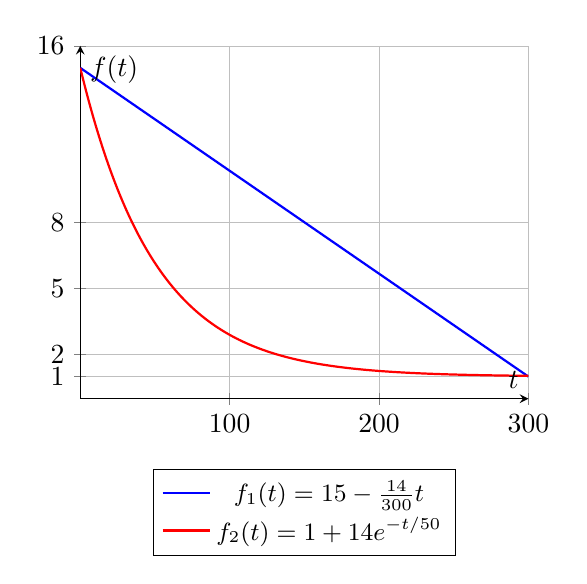
\begin{tikzpicture}
        \begin{axis}[
          width=0.6\linewidth,          % Span the full width of the column
          height=0.5\linewidth,         % Fixed height
          xlabel={$t$},                % Label for the x-axis
          ylabel={$f(t)$},             % Label for the y-axis
          xmin=-0.1, xmax=300,         % Range for x-axis
          ymin=0, ymax=16,             % Range for y-axis
          xtick={0,100,200,300},       % Define specific x-axis ticks      
          ytick={1,2, 5, 8, 16},       % Define specific y-axis ticks      
          grid=both,                   % Display grid lines
          grid style={line width=.1pt, draw=gray!10},
          major grid style={line width=.2pt,draw=gray!50},
          axis lines=middle,           % Position the axes in the middle
          legend style={font=\small, at={(0.5,-0.2)}, anchor=north}, % Position legend below plot
        ]
          % Plotting the Linear Function
          \addplot[
            domain=0:300, 
            samples=300, 
            color=blue, 
            thick
          ]{15 - (14 / 300)*x};
          \addlegendentry{$f_1(t) = 15 - \frac{14}{300} t$}
          
          % Plotting the Exponential Decay Function
          \addplot[
            domain=0:300,
            samples=300,
            color=red,
            thick
          ]{1 + 14 * exp(-x / 50)};
          \addlegendentry{$f_2(t) = 1 + 14 e^{-t/50}$}
        \end{axis}
      \end{tikzpicture}
      % \includegraphics[width=0.49\linewidth]{figures/decrease_length.pdf} \\
    \end{tabular}
    \caption{Adjustement functions used for the dynamic adjustment of action sequence length across time steps.}
    \label{fig:dynamic_adjustment}
\end{figure}


\begin{table}[!htb]
  \centering
  \begin{tabular}{c|c}
  \hline
   & Avg max reward \\
  \hline
  LeRobot & 0.19 \\
  GN & 0.23 \\
  DA (linear) & 0.15  \\
  DA (exponential) & 0.27  \\
  RE (10k) & 0.52 \\
  RE (20k) & \textbf{0.59} \\
  \hline
  \end{tabular}
  \caption{Average max reward of the proposed stragies to overcome the black patch problem.
  "LeRobot" result is the average max reward of the Hugging Face LeRobot model.}
  \label{tab:res_ov_patch}
\end{table}

Table~\ref{tab:res_ov_patch} results demonstrate the effectiveness of data augmentation in significantly improving the model's robustness.
Indeed, we obtain average max reward values similar to those achieved when training the model for 5k steps
without augmentations and evaluating it on unperturbed images (around 0.6).
Additionally, the analysis reveals that even with fewer training steps, the model retains an acceptable performance level, offering a computationally efficient alternative.
\section{Recovering the multimodality}

In Section \ref{sec:action_multimodality}, we highlighted the difficulty of DP in modeling
the multimodal distribution of actions.
More specifically, we concluded that the method's suboptimality was due to non-expert and potentially
biased human demonstrations.
To address this, as we do not have access to expert demonstrations,
we decided to generate new trajectories to create a larger and more diverse dataset.
We first practiced on the PushT task before creating 50 new demonstrations each to reduce biases.
Once the new dataset was complete, we trained the model on these over 300 trajectories for 20k steps.

The effect of these new trajectories was immediate.
In Figure \ref{fig:multimodality_new}, we reproduced the previous singular case and generated 16
different trajectories from different noise vectors.
This time, we clearly see both trajectories emerging on either side of the T.
\begin{figure}[!htb]
    \centering
    \includegraphics[width=0.6\linewidth]{figures/trajectories_multimodality.png}
    \caption{Illustration of the multimodal distribution of actions.}
    \label{fig:multimodality_new}
\end{figure}
To conclude on multimodality, DP is indeed capable of handling situations where multiple actions are possible,
unlike methods that rely on an L2 loss. However, the key to effectively modeling a multimodal distribution
lies in the training data. When a simulator is available, one option could be to generate new data
from existing data by applying geometric transformations or leveraging an expert policy trained through RL.
\section{Conclusion}
\label{sec:conclusion}
This work explores the capabilities and limitations of diffusion policies for visuomotor tasks, specifically within the PushT environment, leveraging the LeRobot framework.
Our experiments confirm the potential of diffusion-based policies for sampling trajectories from a
high-dimensional and multimodal distribution while ensuring temporal consistency.
However, our analysis reveals significant vulnerabilities under out of distribution inputs, such as
visual occlusion, and limitations in showing action multimodality behaviors.

Our results highlight that adding data augmentation leads to noticeable performance improvements, even with 10 times fewer training steps, by evaluating the policy using an alternative metric,
(the coverage rate instead of the success rate).
More generally, as it is challenging to cover all scenarios encountered in reality, it may be beneficial
to detect when the agent faces a situation outside the training distribution. This could involve a module
on top of the policy that identifies the agent's fuzzy movements, often linked to uncertainty in generation.
In this context, we were interested in estimating prediction uncertainty from a batch of generated trajectories.
Our intuition was that in a novel situation, DP would be unable to accurately generate a trajectory,
and the uncertainty would be reflected in the spread of the batch predictions.
Furthermore, to distinguish between multimodality and uncertainty, we considered extracting trends from batch
predictions, for instance, through clustering.
Unfortunately, we observed excessive confidence in trajectory predictions, even in novel situations.

% \todo{Opening on action multimodality:}
% Our findings emphasize the lack of scenarios where the diffusion policy exhibits multimodality behaviors.
% We hypothesize that this limitation could come from the PushT environment itself, which may inherently constrain opportunities for such scenarios, or from insufficient diversity in the dataset.
% Further studies are necessary to investigate this issue and identify potential solutions to encourage and effectively capture multimodal action behaviors.

Regarding action multimodality, we highlighted DP's ability to handle ambiguous situations as well as the
sensitivity of training to the quantity and diversity of data in modeling the underlying multimodal distribution.
More broadly, this issue is linked to the suboptimality of learning from human demonstrations.
Several techniques could help address this problem, including data augmentation, generating expert trajectories
in simulation, or fine-tuning the policy through RL \cite{uehara_understanding_2024,ren_diffusion_2024}.

\newpage
{
    \small
    \bibliographystyle{ieeenat_fullname}
    \bibliography{main}
}

% WARNING: do not forget to delete the supplementary pages from your submission 
% \input{sec/X_suppl}

\end{document}
